\chapter{Planteamiento del problema y revisión de la literatura}\label{Chapter:Introduccion}

\section{Planteamiento del problema}\label{sec:planteamiento}

\noindent La rítmica es una de las partes más importantes de la música. Una misma pieza puede aportar una sensación completamente distinta a un oyente simplemente cambiando el tempo o el ritmo de ésta  \cite{DBLP:journals/corr/abs-1804-08167}. Hasta el resurgimiento de los modelos de aprendizaje profundo los modelos de extracción de información musical (MIR por sus siglas inglesas) se han basado en transformaciones de las señales de audio; estas transformaciones se basan en procesos que requieren tener una gran longitud del audio o pre-procesamiento y creación manual de características para su modelado. Añadido a la complejidad del problema, el diseño de los procesos de extracción de características requiere un amplio conocimiento musical \cite{humphrey:2012}. El problema surge cuando se quiere inferir información de un audio con una longitud más corta (3 segundos por ejemplo), ya sea por disponibilidad o porque se quiera obtener la información más rápidamente sin necesidad de ser experto en características musicales.

En este trabajo se propone el siguiente problema: Predicción de ritmos dada una corta grabación para ayudar en la elección de una base rítmica. Actualmente lo que haría un músico (o productor) para solucionar esto es probar con varios ritmos utilizando conocimiento previo hasta que uno encaje, esto además requiere que se genere la base rítmica. Sin embargo, un sistema automático podría rápidamente detectar un tempo y predecir un ritmo adecuado. Dados los requisitos del problema y la disponibilidad de recursos se simplificará el problema a una clasificación de género y predicción de tempo, ya que estas dos características son principales determinantes del ritmo de  una canción. 

En el siguiente apartado se va a presentar una revisión literaria del estado de la clasificación musical a través de aprendizaje profundo.

\section{Revisión literaria}\label{sec:revision}

\noindent Los primeros trabajos de redes neuronales con música aparecieron en 1988 y generaron una época de composición musical algorítmica que duró hasta 2009 sobreviviendo el invierno de la inteligencia artificial \citep{Pons:TowardsDataScience2018}. Una de las propuestas que inició el movimiento fue una red profunda (dos capas ocultas y una capa de salida) en la que los autores defienden que este tipo de redes son capaces de generar resultados artísticos originales a partir de suficientes datos \citep{lewis:1988}. Por otro lado \cite{Todd1988} propuso una red recurrente (RNN) para generar música de manera secuencial. Esta tendencia a usar redes secuenciales es la que ha isnpirado el movimiento \citep{Pons:TowardsDataScience2018} y los resultados han ido mejorado al hacer uso de células LSTM \citep{eck:temporalstructure:2002}.

\begin{figure}[htb]
  \centering
  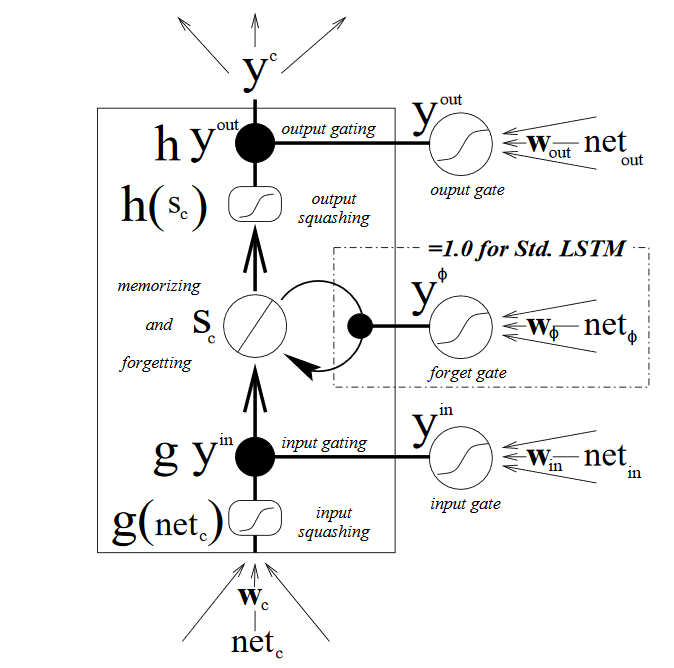
\includegraphics[width=0.4\textwidth]{Figures/lstm_cell.png}
  \caption{\textcolor{black}{Diseño de una neurona LSTM de \cite{Gers2000LearningTF,Gers2001LSTM}}.}
  \label{Fig:lstm_cell}
\end{figure}

\cite{eck:temporalstructure:2002} comentan que, aunque las redes recurrentes (RNN) se hayan utilizado para generar música, éstas tienen un defecto y éste es que la música generada por RNN suele tener falta de coherencia global como la que suele estar presente en música real. Ésto se debe a que las redes neuronales recurrentes (RNN) suelen tener problemas de gradientes desvanecedoras. Una manera de hacer que una red temporal recuerde eventos pasados sin problemas de gradiente es utilizando neuronas LSTM (Figura~\ref{Fig:lstm_cell}). \cite{eck:temporalstructure:2002} proponen una red LSTM para generar música automáticamente, específicamente componen un Blues de 12 compases. En sus estudios descubren que una red secuencial basada en neuronas LSTM no se desvía de la estructura principal de la pieza y consigue componer blues con buen tiempo y estructura.

Recientemente ha habido un cambio importante en el campo de MIR con la introducción de los procesadores gráficos (GPU) y las redes convolucionales (CNN). En 2009 se presentó una investigación que muestra que las representaciones de características creadas por redes convolucionales sobrepasaba la efectividad de características usadas hasta el momento en procesamiento de audio \citep{Lee:2009}. En su investigación, \cite{Lee:2009} aplican estos resultados para el diseño de redes profundas \textit{Deep Belief} (CDBN) y presentan resultados prometedores en el campo de clasificación musical (para etiquetado de género y artista).

Mientras que la extracción de información musical clásica requiere la construcción de características a partir de señales de audio o creación de meta-datos, el procesamiento de música con redes profundas se puede realizar con muchos tipos de datos. Entre ellos se encuentran: representaciones textuales de música escrita, representaciones visuales de música escrita, audios puros, audios pre-procesados y representaciones visuales de audios. En el campo del aprendizaje profundo y de cara a información extraída de audios reales se han utilizado audios y representaciones visuales de audios principalmente. Las representaciones de audios utilizadas son los espectrogramas de coefficientes \textit{Cepstral} (MFCC). Éstos son mapas de intensidad de frecuencia con respecto del tiempo, normalmente representándose el tiempo en el eje `x', la frecuencia en el eje `y' y la intensidad en el eje `z' (generalmente representada en color). Éste tipo de representaciones son las más usadas por modelos CNN. 

\begin{figure}[htb]
  \centering
  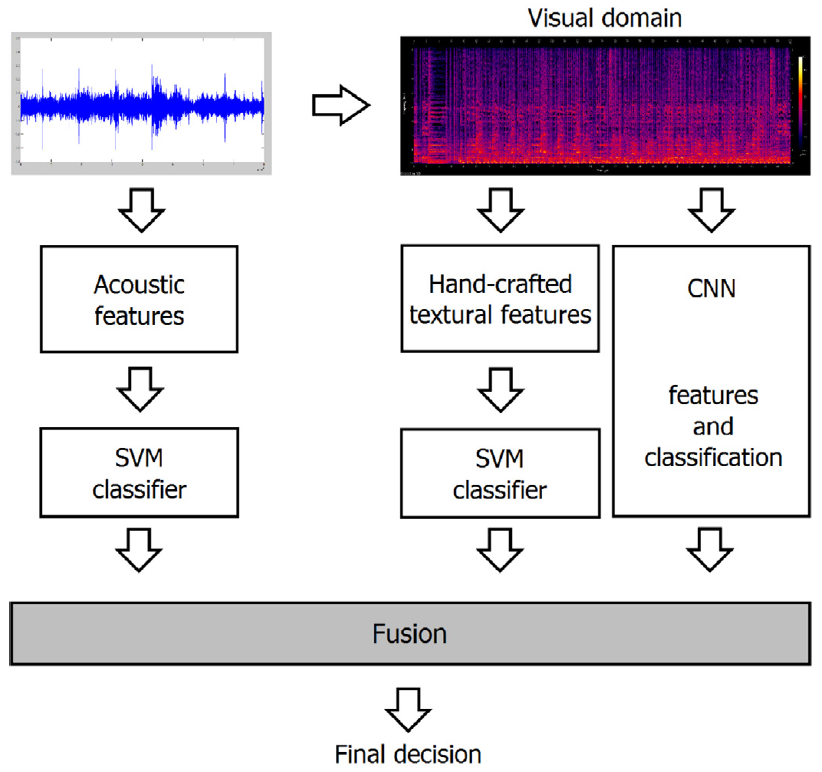
\includegraphics[width=0.6\textwidth]{Figures/audio-spectrogram_model_costa2017.png}
  \caption{\textcolor{black}{Modelo de clasificación utilizando ambos audio y representación de espectrograma por \cite{MGCosta:softcomputing:2017}}.}
  \label{Fig:audio-spectrogram_model_costa2017}
\end{figure} 

Para comparar un modelo clásico con uno profundo, \cite{MGCosta:softcomputing:2017} presentan un etiquetador de género  comparando el uso de espectrogramas (con y sin cálculo manual de características) y audio sin procesar. Además proponen un modelo de conjunto que utilice los tres métodos para mejorar la precisión (Figura~\ref{Fig:audio-spectrogram_model_costa2017}). Para sus predicciones utilizan el set de datos ISMIR (http://www.ismir.net/resources/datasets/), el cual será útil más adelante cuando se necesiten datos de entrenamiento.

En su investigación descubren que el clasificador entrenado en representaciones visuales (espectrogramas) tiene un mejor desempeño que clasificadores entrenados con representaciones sonoras y características manufacturadas.

Estos resultados son parcialmente afines a los resultados por \cite{pons:end2end:2018} y \cite{Lee:2009}. Sin embargo, \cite{pons:end2end:2018} concluyen que la diferencia entre los modelos basados en audio y los modelos basados en espectrogramas se diferencian principalmente en la cantidad de datos y la cantidad de pre-procesamiento de estos. Cuando hay pocos datos disponibles (100k canciones de entrenamiento) es necesario el pre-procesamiento de los datos para un buen funcionamiento de los modelos y en este caso las redes convolucionales destacan. Usando conocimientos musicales uno puede diseñar los filtros de las convoluciones para extraer la información deseada por lo tanto haciendo un modelo más específico y eficiente para la tarea planteada. Por otro lado, cuando la cantidad de datos más grande (1M canciones de entrenamiento) un modelo basado en audio puro supera los modelos basados en espectrogramas.

Además de su investigación sobre la eficiencia de las redes convolucionales, \cite{pons:end2end:2018} realizan una revisión de los modelos actuales y proponen una arquitectura típica para modelos de extracción de información musical (Figura~\ref{Fig:deeplearningpipeline_pons2018}).

\begin{figure}[htb]
  \centering
  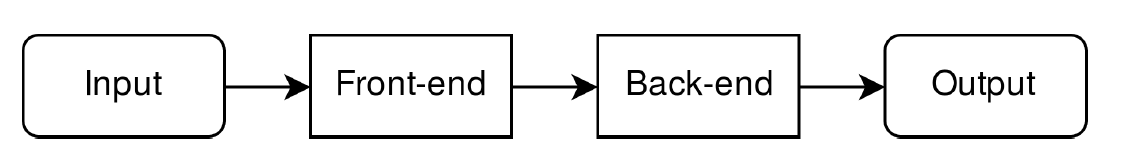
\includegraphics[width=0.7\textwidth]{Figures/deeplearningpipeline_pons2018.png}
  \caption{\textcolor{black}{Arquitectura general de un modelo de extracción de información musical definida por \cite{pons:end2end:2018}}.}
  \label{Fig:deeplearningpipeline_pons2018}
\end{figure}

\cite{pons:end2end:2018} identifican que la arquitectura principal que se está utilizando para clasificación de audio está principalmente dividida en ``Input", ``Front-end", ``Back-end"{ } y ``Output" (Figura~\ref{Fig:deeplearningpipeline_pons2018}) y estas se constituyen de lo siguiente:
\begin{itemize}
\item \textbf{Input:} estructura de datos que acepte el modelo (audio, espectrograma, meta-datos).
\item \textbf{Front-end:} extracción de características, generalmente a través de capas convolucionales.
\item \textbf{Back-end:} Procesamiento de características (capas densas) que tienen que poder admitir entradas de tamaño variable en ciertas ocasiones. Lo último se puede conseguir mediante capas de pooling o capas recurrentes, por ejemplo LSTMs (neuronas de Long-Short Term Memory)
\item \textbf{Output:} El output es la clasificación o etiquetado del modelo.
\end{itemize}

Retomando el tema de la preferencia del MIR por las CNN: recientemente se ha estado identificando que la razón principal por la que las redes convolucionales fallan al clasificar imágenes es porque éstas ven principalmente texturas donde el ser humano ve formas. Sin embargo, esta preferencia por las CNN de ver texturas en imágenes ha sido aprovechada en el campo de extracción de información musical para determinar el tipo de sonido (o tipo de instrumentos) en una pieza. \cite{Han:instrumentRecognition:2017} presentan una red convolucional (Figura~\ref{Fig:CNN_instrument2017}) para clasificar el instrumento predominante en un audio. 

\begin{figure}[htb]
  \centering
  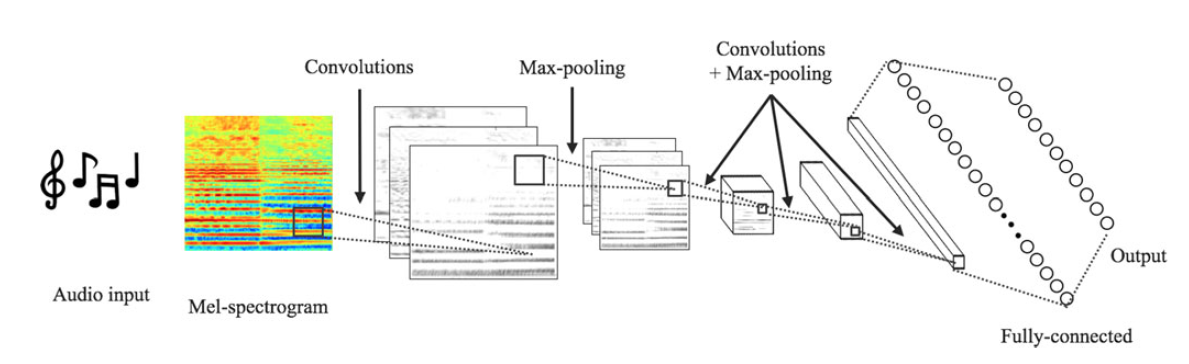
\includegraphics[width=0.9\textwidth]{Figures/CNN_instrument2017.png}
  \caption{\textcolor{black}{Red Convolucional para clasificación de instrumento por \cite{Han:instrumentRecognition:2017}}.}
  \label{Fig:CNN_instrument2017}
\end{figure}

La clasificación de instrumentos con espectrogramas es posible ya que, para una misma nota, distintos instrumentos tienen distinto timbre. Ésto significa que las frecuencias resonantes dominantes serán distintas para cada instrumento y esto se verá como un patrón dentro del espectrograma; la red convolucional es capaz de extraer estas texturas o patrones gracias a los filtros aplicados. \cite{Han:instrumentRecognition:2017} defienden que sus experimentos consiguen una mejora del $\approx20\%$ sobre algoritmos del estado del arte al comparar métricas F1 en este tipo de clasificadores. También concluyen que para el diseño de las capas convolucionales es necesario un conocimiento musical para saber que características se están extrayendo. \cite{Han:instrumentRecognition:2017} también encuentran que, al igual que en redes profundas, la primera capa de convoluciones está extrayendo características simples (en este caso líneas verticales y horizontales) y el resto de capas se activan con patrones más complejos.

\cite{DBLP:journals/corr/PonsSGGS17} también investigan el uso de la extracción del timbre en espectrogramas con el fin de resolver tareas de clasificación/etiquetado de audio musical y de audio general. En su artículo investigan como el diseño de los filtros y capas convolucionales ayudan a diseñar una red para la tarea en mente. A consecuencia de esto proponen unas pautas para diseñar redes CNN para clasificación de música. Por ejemplo proponen que filtros pequeños son buenos para la eficiencia en general del modelo además de ser óptimos para activar frecuencias de bajo o bombo de la batería. También denotan que para capturar sonidos de percusión es necesario detectar formas llanas (horizontales) en las representaciones espectrales. ésta información es de gran utilidad para poder diseñar una red CNN que capture ritmos.

Por otro lado, para la correcta extracción de ritmos de un audio, un sistema de extracción musical debe acertar el ritmo independientemente del tempo de éste, esto significa que no solo es necesario captar percusiones en el espectrograma si no que es necesario que infiera el tempo o contexto temporal. \cite{DBLP:journals/corr/abs-1804-08167} presenta la idea de que las redes convolucionales pueden detectar distintos ritmos de un audio independientemente del tempo de dicho audio.

En su análisis, \cite{DBLP:journals/corr/abs-1804-08167} propone que hay distintos tipos de variabilidades con respecto al tiempo en la música y un sistema de extracción de información de música debe tener una serie de invariabilidades con respecto a las características de una pieza. Los tipos de invariabilidades posibles se muestran en la tabla~\ref{tab:invariance_rythms}. 

\begin{table}
\centering
\begin{tabular}{ll}
\hline
\textbf{Invariabilidad} & \textbf{Descripción}                                                  \\ \hline
Tempo                   & Invariable con respecto al tempo                                      \\
Fase                    & Invariable con respecto a la fase del ritmo \\
Ritmo                   & Invariable con respecto al tempo y a la fase                          \\
Pulso                   & Invariable con respecto a un pulso predeterminado                     \\
``Cepstroid"            & Invariable con respecto a la repetición dominante de la canción  \\
Tiempo                  & Invariable con respecto al tiempo                                     \\
Tono                    & Invariable con respecto a la frecuencia                               \\ \hline
\end{tabular}
\caption{\textcolor{black}{Invariabilidades a tener en cuenta para el procesamiento de ritmo en música, de \cite{DBLP:journals/corr/abs-1804-08167}}}
\label{tab:invariance_rythms}
\end{table}

El ritmo musical y el tempo (o métrica) son especialmente importantes porque ofrecen un contexto en el que el oyente puede interpretar la estructura y melodías de una pieza. \cite{DBLP:journals/corr/abs-1804-08167} pone como ejemplo una nota que ocurre a los 0.125 segundos del comienzo de un compás musical. En una pieza que tenga de tempo 120 pulsaciones por minuto esta nota estaría a una distancia de una semicorchea ($1/16$ pulsos) del inicio, en una pieza de 160 pulsaciones por minuto la nota estaría a una distancia de una corchea con puntillo ($3/16$ pulsos) del inicio. 

Por otro lado, la estructura del ritmo en la música es importante y suele estar muy definida globalmente en una pieza. por ejemplo: la música rock popular suele tener \setmeterb{4}{4} (4 pulsos por compás), pero un vals tiene una métrica de \setmeterb{3}{4} (3 pulsos por compás). Esto significa que cambios melódicos importantes suelen ocurrir cada cuatro pulsos en el rock y cada 3 en un vals \citep{eck:temporalstructure:2002}

Basado en esto la literatura muestra que las redes convolucionales han sido elegidas para el procesamiento de información musical gracias a sus propiedades de Invariabilidad-tiempo e invariabilidad-tono. Esto es gracias al uso de convoluciones idénticas en distintas zonas de una representación gráfica/linear de un clip de audio: Eventos repetidos temporalmente pueden ser captados por convoluciones a lo largo de la dimensión del tiempo, mientras que convoluciones con respecto a la frecuencia puede captar ritmos en distintas frecuencias o tonos \citep{DBLP:journals/corr/abs-1804-08167}.

\cite{DBLP:journals/corr/abs-1804-08167} encuentra que cambiando de los tipos de filtros usados en la última capa antes de las capas densas de la red se puede optimizar la red para distintas tareas. Entre ellas distinguen: género musical, correlación de patrones, complejidad rítmica, claridad rítmica, métrica, detección de infracciones de copyright y \textit{swing} (estilo de ritmo típico de Jazz y Blues). Sin embargo, las investigaciones de este artículo se realizan sobre audios simplificados de ritmo, por lo que solo son representativos del potencial de la técnica y más trabajo es necesario en éste area.

Las redes convolucionales han demostrado una gran eficiencia prediciendo el género musical de audios, pero hacer predicciones de tempo, aún teóricamente posible segun los resultados de la literatura, ha demostrado ser algo más complicado. Previamente esto se hacía analizando trozos de un audio y superponiendo audios para calcular relaciones temporales \citep{tristan:2005,klapuri:2006} o bien haciendo cálculos avanzados sobre series temporales \citep{sheng:2004}. 

\begin{figure}[htb]
  \centering
  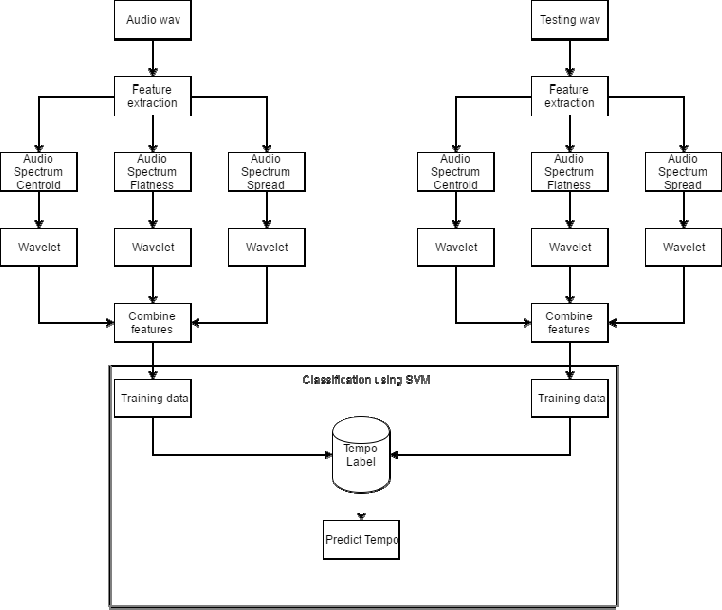
\includegraphics[width=0.7\textwidth]{Figures/system_architecture_Lazaro2017.png}
  \caption{\textcolor{black}{Arquitectura de un predictor de tempos por \cite{Lazaro2017MusicTC}}.}
  \label{Fig:system_architecture_Lazaro2017}
\end{figure}

Un ejemplo a mitad de camino dónde se mezcla la extracción clásica de características y los algoritmos de aprendizaje automático lo dan \cite{Lazaro2017MusicTC}. En su investigación, \cite{Lazaro2017MusicTC} utilizan extracción clásica de características de audio y aplican un algoritmo de aprendizaje automático basado en máquinas de vectores soporte (SVM). Para la extracción de características, usan tres tipos de extracción de características clásicas: centroide del espectro de audio (ASC), llanura del espectro de audio (FSC) y dispersión del espectro de audio (ASS). Estas tres características se sacan haciendo transformaciones de la señal usando principalmente transformaciones de Fourier y logaritmos para extraer frecuencias dominantes de la señal. Posteriormente se pasan las señales alteradas a una máquina de vector soporte como se muestra en el esquema (Figura \ref{Fig:system_architecture_Lazaro2017}).

Para las predicciones, \citeauthor{Lazaro2017MusicTC} transforman los tempos en 3 clases: lento, medio y rápido. Ésta es una simplificación significativa del problema, pero se debe de hacer debido a que el algoritmo usado no sería potente suficiente cómo para separar alrededor de 100 clases con los datos disponibles. Para separar las 3 clases utilizan una máquina de vector soporte (SVM) y consiguen una precisión del $80\%$, éste es un buen resultado pero está todavía bastante alejado de conseguir una predicción del tempo actual precisa. Para realizar ésto necesitaríamos utilizar algoritmos de aprendizaje profundo.

\cite{humphrey:2012} defienden que la creación de características es un proceso en cadena que podría ser simulado por una red profunda y encuentran paralelismos entre la forma que una red convolucional procesa información y la manera clásica de obtener características. Una gran ventaja sobre la extracción clásica que añaden a las ya discutidas es que al seleccionar características podríamos estar desechando otras importantes. Para evitar eso se necesitaría un conocimiento muy profundo del problema y dichas características serían muy especificas para el problema para el que se han diseñado. 

Aunque el problema de la predicción del tempo usando redes convolucionales necesita bastante trabajo, \cite{humphrey:2012} concluyen es posible diseñar un modelo capaz de predecir tempo. No obstante, esto requiere una re-evaluación del problema, ya que éste se ha ido desarrollando para que tenga una solución algorítmica que no es fácilmente adaptable a una red profunda.

Recientemente, \cite{Schreiber:2018} han demostrado que una implementación profunda directa al problema es posible y presentan una investigación donde utilizan una red profunda de capas convolucionales (CNN) para extraer tempo directamente del espectrograma de un audio sin procesar. La red tiene dos características destacables: los filtros que utilizan para procesar el audio son todos horizontales y utilizan módulos multi-filtro (Figura \ref{Fig:system_architecture_Schreiber2018}) en la parte central de la red. Los módulos multi-filtro están compuestos por convoluciones paralelas con diferentes características que son concatenadas posteriormente y pasadas por una convolución final a modo de unión de la capa. Todas las capas están activadas con la función Exponential Linear Unit (ELU).

\begin{figure}[htb]
  \centering
  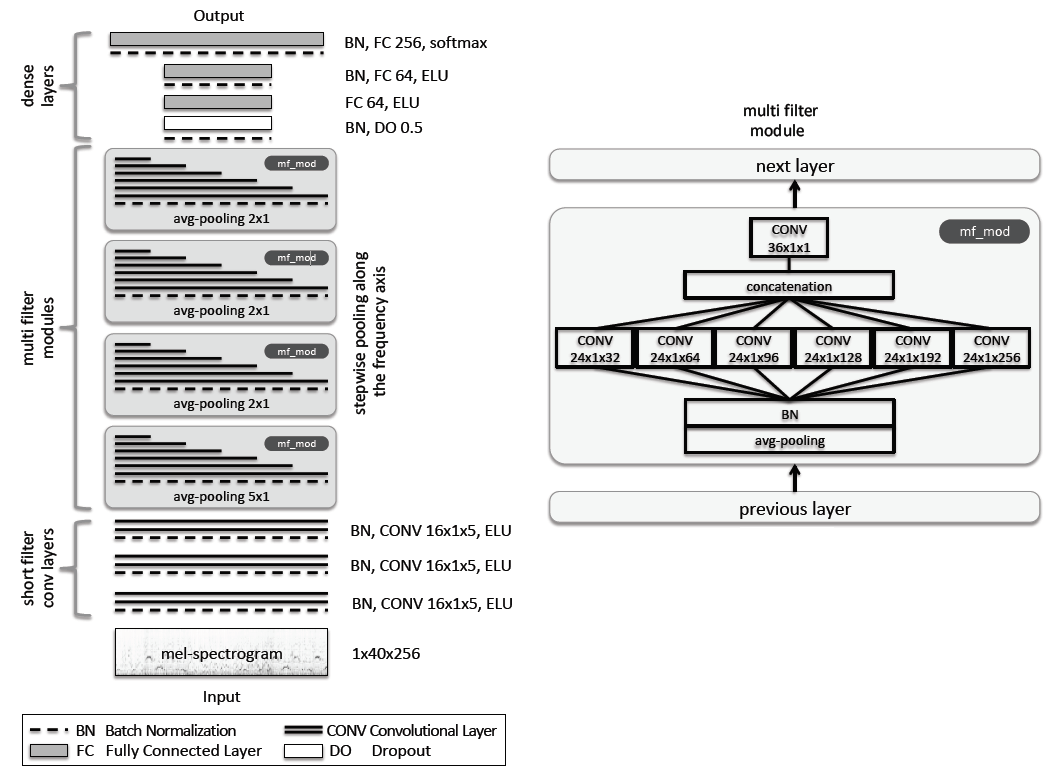
\includegraphics[width=0.9\textwidth]{Figures/system_architecture_Schreiber2018.png}
  \caption{\textcolor{black}{Arquitectura de un predictor de tempos con una red CNN profunda por \cite{Schreiber:2018}}.}
  \label{Fig:system_architecture_Schreiber2018}
\end{figure}

\cite{Schreiber:2018} prueban la red con varios sets de datos y definen tres tipos de precisión para evaluar los resultados: \textit{Accuracy0} es la precisión de predecir el íntegro más cercano del tempo, \textit{Accuracy1} es la precisión permitiendo una desviación del $4\%$ y \textit{Accuracy2} es similar a la anterior pero también permitiendo errores por octava (los errores por octava es la predicción de tempos múltiplos del verdadero por 2 o 3). De media reportan los resultados mostrados en la Tabla \ref{tab:CNN_tempo_shcreiber2018}.

\begin{table}
\centering
\begin{tabular}{ll}
\hline
\textit{Accuracy0}                   & $42.1\%$           \\
\textit{Accuracy1}                   & $69.3\%$           \\
\textit{Accuracy2}                   & $86.4\%$           \\ \hline
\end{tabular}
\caption{\textcolor{black}{Precisiones medias de la red profunda de \cite{Schreiber:2018}}}
\label{tab:CNN_tempo_shcreiber2018}
\end{table}

Como se puede ver en la Tabla \ref{tab:CNN_tempo_shcreiber2018}, la precisión estricta de tempo no es ideal, aunque aumentar una tolerancia del $4\%$ incrementa significativamente la precisión de la red. Los resultados también muestran que la predicción de tempos dobles o triples al actual es bastante común para este tipo de red. \cite{Schreiber:2018} concluyen que los resultados podrían ser mejorados utilizando sets de datos más balanceados o bien mejorando la arquitectura de la red. Entre las propuestas sugieren filtros más cortos en las convoluciones y capas densas más grandes.


\section{Propuesta de modelo}\label{sec:propuesta}

\noindent La revisión literaria del estado actual de la extracción de información musical (MIR) sugiere que es posible diseñar un modelo que sea capaz de predecir tanto género como tempo a partir de un audio convertido a espectrograma. Las redes convolucionales han sido demostradas como eficientes para el problema planteado, aunque las predicciones de tempo no son todavía completamente satisfactorias. 

Usando la información recogida en esta sección se van a proponer unas cuantas arquitecturas de redes convolucionales para predecir género y tempo y se intentará mezclar estas arquitecturas en una sola red. La idea de estos experimentos es, demostrar la posibilidad de extraer ritmos de un audio con un modelo único utilizando dichas herramientas. 